\chapter{Практическая часть}
\label{cha:pract}

\section{Постановка задачи}

В рамках практической части работы, было выделены следующие задачи:

\begin{itemize}
 \item изучить средства разработки программного обеспечения для микрокотроллеров семейства ARM;
 \item адаптировать существующее открытое программное обеспечение к другой аппаратной платформе;
 \item создать работающие прототипы конечных устройств с трансиверами LoRa;
\end{itemize}

\section{Выбор аппаратной платформы}

\subsection{STM32L476G-Discovery}

Для разработки конечных устройств была выбрана отладочная плата STM32L476G-Discovery на базе 32-битного микроконтроллера STM32L476VGT6 с ядром ARM-Cortex M4.
Данный микроконтроллер является представителем семейства микроконтроллеров с низким энергопотреблением STM32L4 фирмы ARM.
Микроконтроллер имеет:
\begin{itemize}
 \item 3 устройства I2C;
 \item 3 устройства SPI;
 \item поддержка шины CAN;
 \item SWPMI;
 \item 2 x SAI;
 \item 12-битное ЦАП;
 \item драйвер LCD;
 \item 128 Кбайт SRAM;
 \item 1 МБайт Flash;
 \item Quad-SPI;
 \item touch sensing;
 \item USB OTG FS;
 \item поддержка JTAG отладки;
\end{itemize}

Удобство данной отладочной платы заключается в том, что вся необходимая вспомогательная периферия уже находится на плате, и подключена ко входам и выходам микроконтроллера.
В качестве вспомогательной периферии служат:

\begin{itemize}
 \item программатор/отладчик ST-LINK/V2-1;
 \item LCD дисплей;
 \item кнопка RESET;
 \item джойстик;
 \item встроенный амперметр, для измерения тока потребления микроконтроллера в режиме low power;
 \item USB OTG FS;
 \item аудио ЦАП;
 \item MEMS (микрофон, 3-осевой гироскоп, 6-осевой компас);
 \item Quad-SPI Flash память;
 \item светодиоды.
\end{itemize}

Вид на плату сверху отображён на рисунке \ref{fig:discovery}.

\begin{figure}[!h]
  \centering
  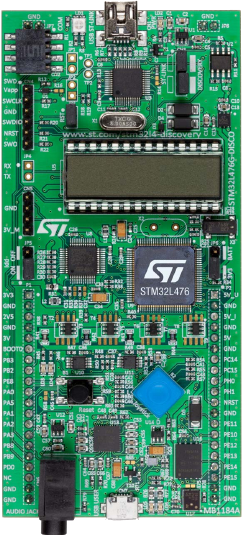
\includegraphics[height=0.3\textheight]{inc/img/discovery}
  \caption{Отладочная плата STM32L476G-Discovery}
  \label{fig:discovery}
\end{figure}

\subsection{Трансивер LoRa SX1278}

Выбор данного трансивера был обусловлен тем, что он уже имелся в наличии и его внутренняя структура схожа с трансивером SX1272 (они имеют общее руководство по эксплуатации).

Раздел в процессе написания...

\begin{figure}[!h]
  \centering
  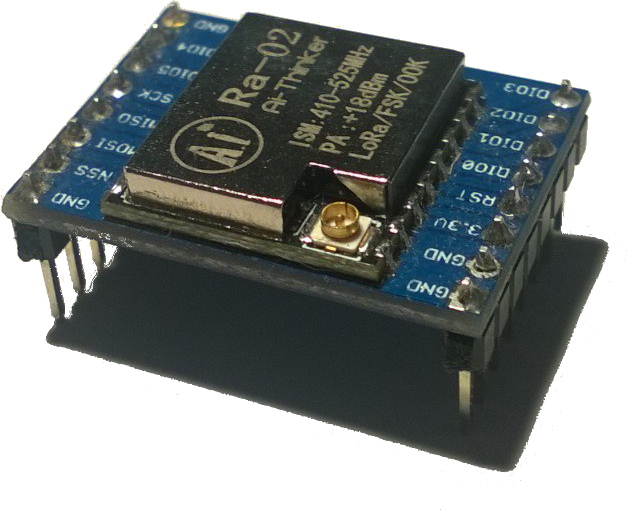
\includegraphics[height=0.3\textheight]{inc/img/SX1278}
  \caption{Трансивер SX1278}
  \label{fig:sx1278}
\end{figure}

\section{Выбор средств разработки}

Раздел в процессе написания...
%Зачем взял LoRaMac на гитхабе
%Возможно немного слов про открытое ПО
%Ещё чуть чуть про инструменты

\subsection{CMake}

Раздел в процессе написания...

\subsection{HAL}

Раздел в процессе написания...

\subsection{Выбор компилятора для STM32}

Раздел в процессе написания...

\subsection{ST-LINK и Openocd}

Раздел в процессе написания...

\begin{figure}[!h]
  \centering
  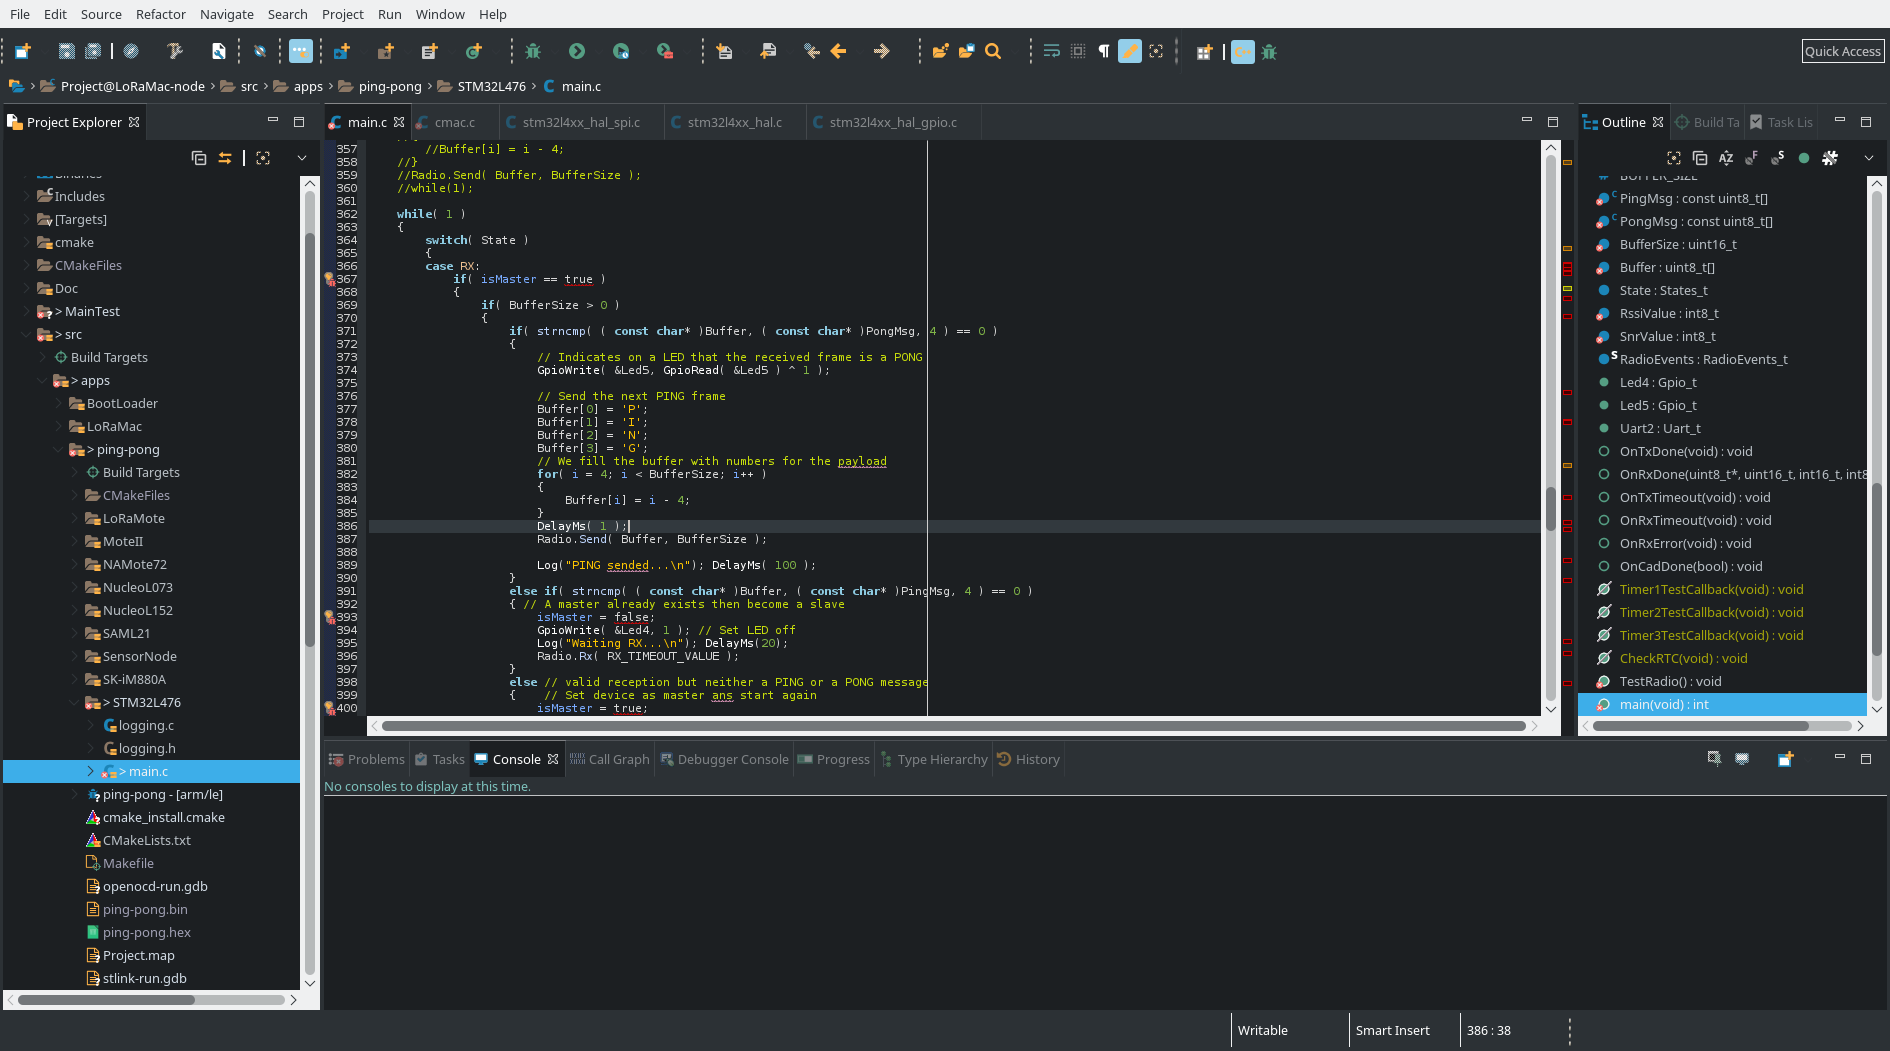
\includegraphics[width=\textwidth]{inc/img/EclipseSTM}
  \caption{Интегрированная среда разработки CDT Eclipse}
  \label{fig:ideeclipse}
\end{figure}


\begin{listing}[H]
 
\end{listing}
\label{lst:boardinit}

\subsection{Структура проекта LoRaMac}
%Правила переноса кода
\begin{figure}[!h]
  \centering
  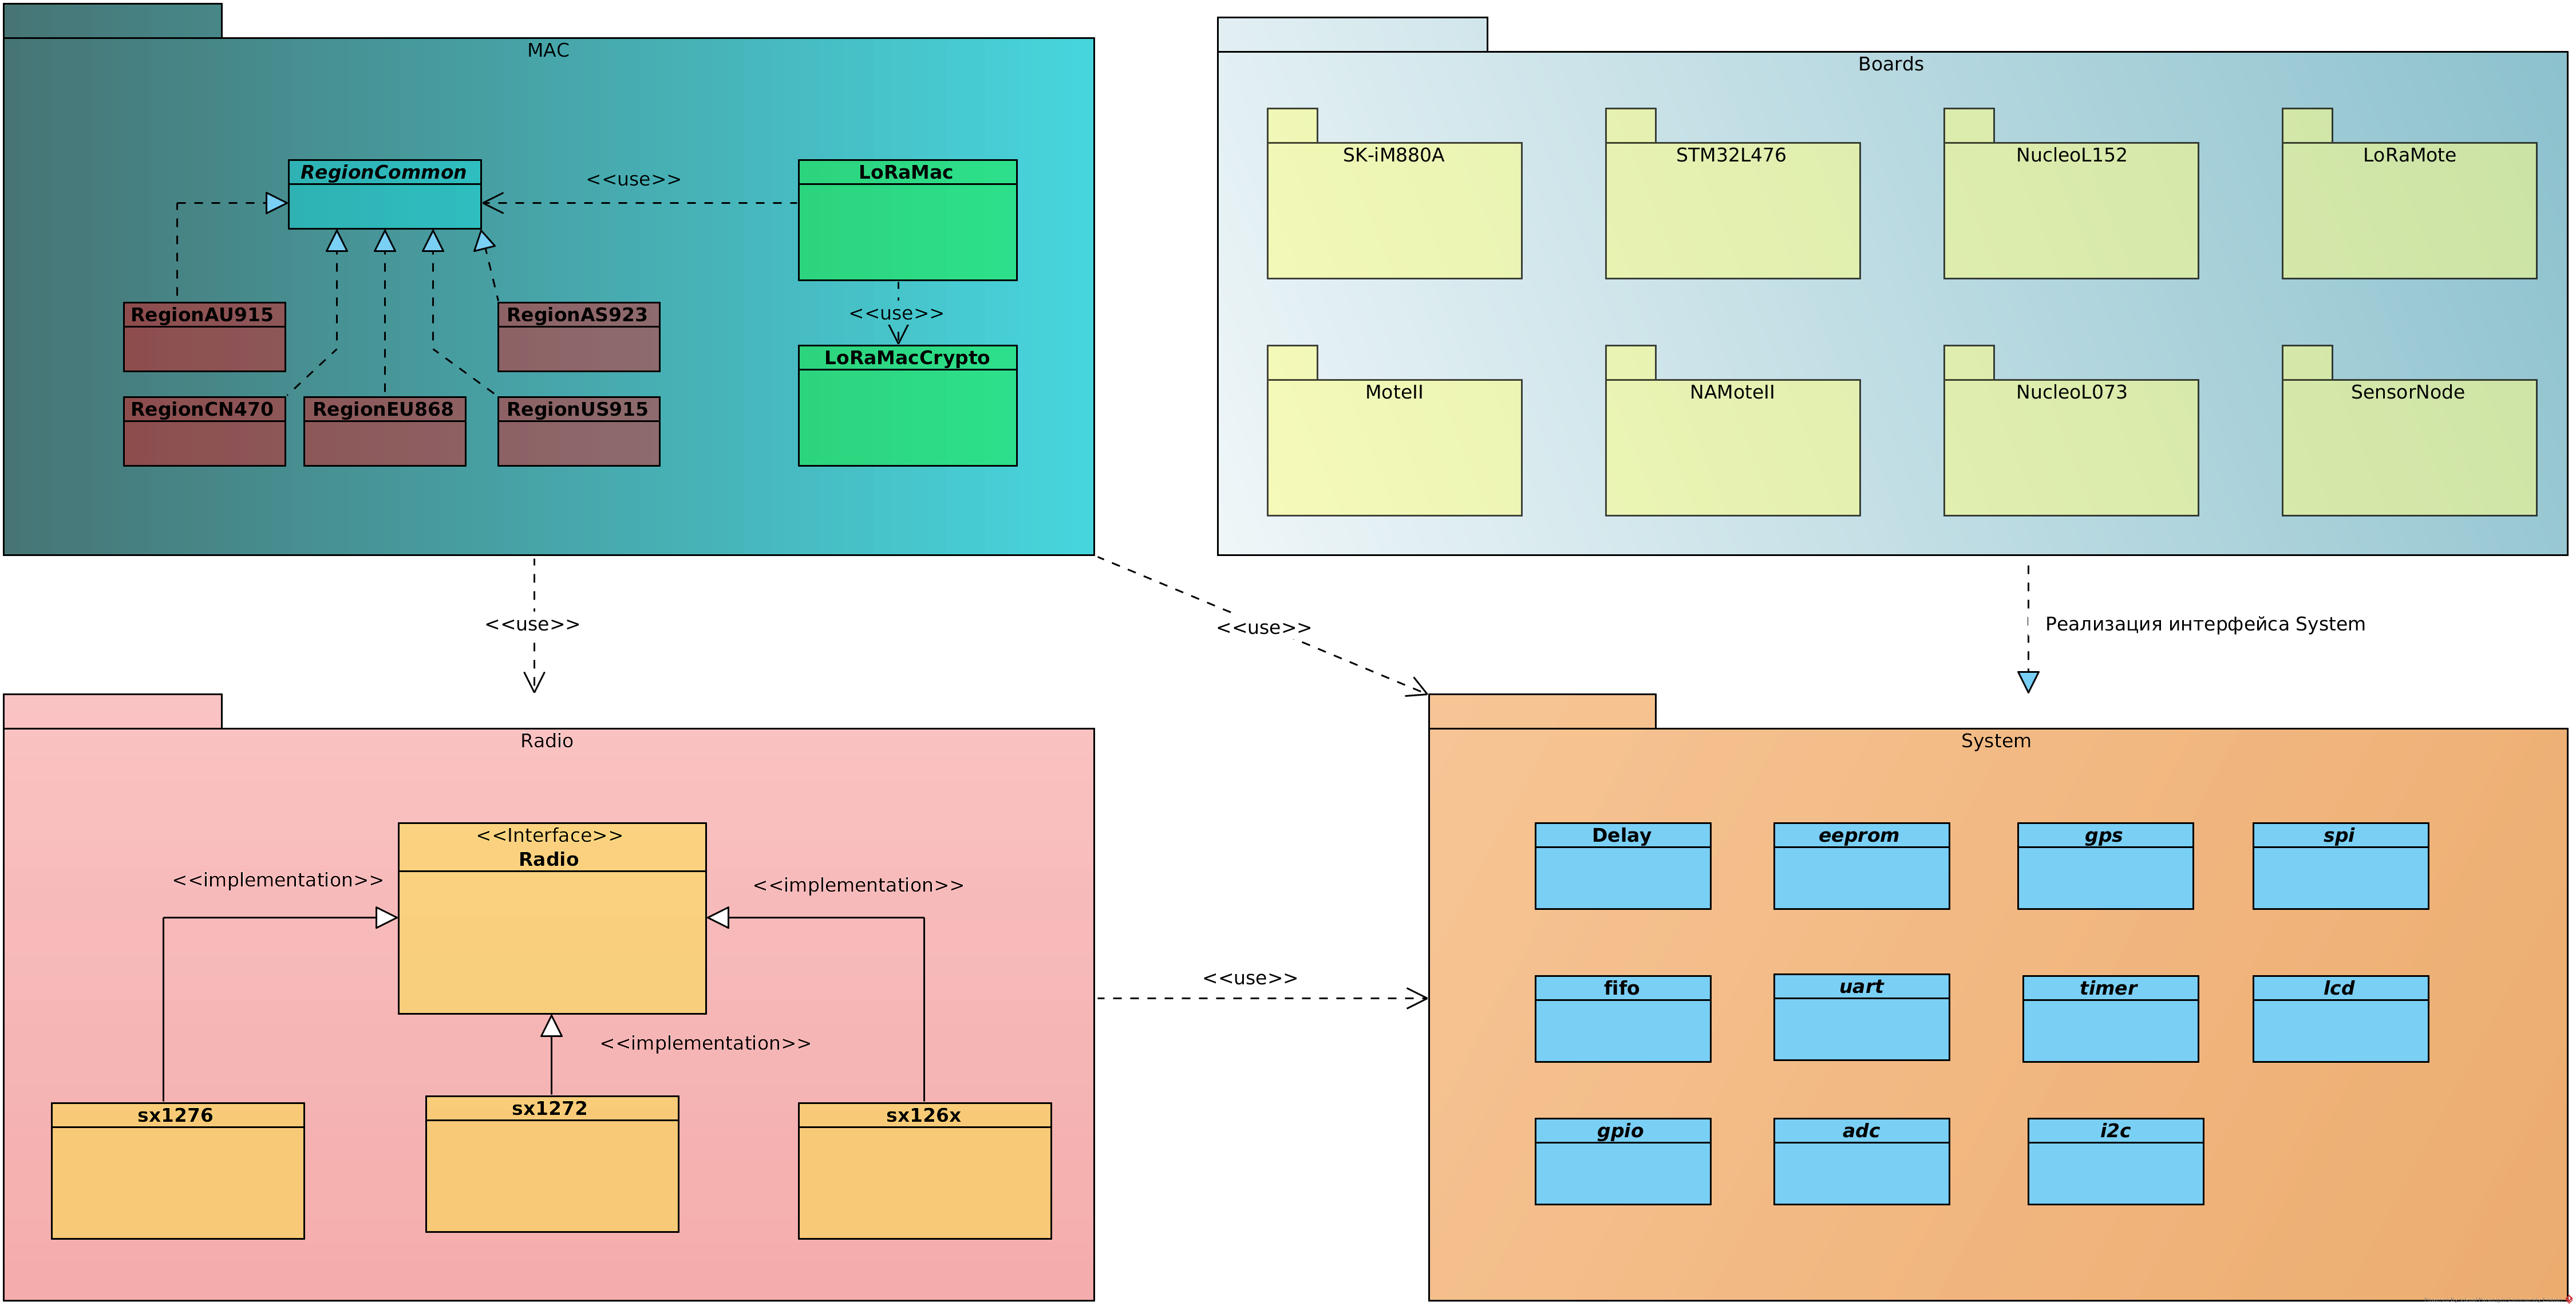
\includegraphics[width=\textwidth]{inc/img/LoRaMacProj}
  \caption{Упрощенная структура проекта LoRaMAC в нотации UML}
  \label{fig:loramacstructure}
\end{figure}

\begin{listing}[H]
% firstline, lastline - какие строки показывать 
\cmakefile{inc/src/CMakeLists.txt}
\caption{Основной CMakeLists} 
\end{listing}
\label{lst:maincmake}

\section{Реализация проекта}

Раздел в процессе написания...

\subsection{Подключение STM32 к трансиверам LoRa}
Раздел в процессе написания...

% Желательно схему

\subsection{Трудности переноса}
Раздел в процессе написания...

% Вспомни про несовместимость HAL и LoRaMac

\subsection{Компиляция и отладка}
Раздел в процессе написания...

%\begin{listing}[H]
% firstline, lastline - какие строки показывать 
%\cfile{inc/src/test.c}
%\caption{Пример — test.c} 
%\end{listing}
%\label{lst:c}

%Можно также использовать окружение \Code{verbatim}, если \Code{listings} чем-то не
%устраивает. Только следует помнить, что табы в нём <<съедаются>>. Существует так же команда \Code{\textbackslash{}verbatiminput} для вставки файла.

%\begin{verbatim}
%a_b = a + b; // русский комментарий
%if (a_b > 0)
    %a_b = 0;
%\end{verbatim}

%%% Local Variables:
%%% mode: latex
%%% TeX-master: "rpz"
%%% End:
